\documentclass[a4paper,11pt,british,DIVcalc]{scrartcl}
\usepackage[T1]{fontenc,url}
\usepackage[latin1]{inputenc}
\usepackage{soul,babel,mflogo,xspace,tabularx,fancyref,booktabs,textcomp,ifpdf}
\usepackage[dvips]{graphicx}
\usepackage[final]{listings}
\usepackage[sc]{mathpazo}
%\usepackage{luximono}


\newcommand{\exteps}{\texttt{\upshape exteps}\xspace}
\newcommand{\delfin}{\texttt{\upshape delfin}\xspace}
%\let\delfin\relax

\usepackage{hyperref}
\addto\itemize{\def\labelitemi{-\kern-.15em-}}
\hypersetup{ps2pdf,a4paper,pdfauthor=Palle J�rgensen, pdftitle={exteps
    documentation}, pdfsubject={Inclusion of external EPS graphics in
    MetaPost figures},pdfkeywords={MetaPost,EPS,external,exteps}}
\author{Palle J�rgensen} 

\title{\so{Using external EPS graphics in} \MP\\\LARGE \so{The}
  \exteps \so{module}\\\so{Version} \oldstylenums{0.41}}

\lstset{basicstyle=\small,breaklines=true,columns=fullflexible}
\renewcommand{\thesection}{\oldstylenums{\arabic{section}}}
\renewcommand{\thesubsection}{\oldstylenums{\arabic{subsection}}}
\renewcommand{\thefigure}{\oldstylenums{\arabic{figure}}}
\renewcommand{\thepage}{\oldstylenums{\arabic{page}}}

\makeatletter
\let\vref@space\space
\let\old@section\section
\def\section{%
  \@ifstar{%
    \old@section*%
  }{%
    \so@section}%
}
\def\so@@@section#1{\old@section[#1]{\so{#1}}}
\def\so@@section[#1]#2{\old@section[#1]{\so{#2}}}
\def\so@section{%
  \@ifnextchar[%]
  {%
    \so@@section
  }{%
    \so@@@section
  }%
}

\let\old@subsection\subsection
\def\subsection{%
  \@ifstar{%
    \old@subsection*%
  }{%
    \so@subsection}%
}
\def\so@@subsection[#1]#2{\old@subsection[#1]{\so{#2}}}
\def\so@@@subsection#1{\old@subsection[#1]{\so{#1}}}
\def\so@subsection{%
  \@ifnextchar[%]
  {%
    \so@@subsection
  }{%
    \so@@@subsection
  }%
}
\def\trr{\rightskip\@flushglue}

\makeatother
\renewcommand{\textfraction}{0}
\addtokomafont{sectioning}{\normalfont\scshape}
\lstset{language=metapost}

\begin{document}
\def\contentsname{\so{Contents}}
\maketitle
\tableofcontents

\clearpage
\section{Introduction}
\label{sec:introduction}

This document describes the use of the \exteps module for inclusion of
external EPS figures in \MP\ figures. Unlike the previous attempt
(epsincl) it make no use external programs\footnote{This is only
  partly true, as \MP\ is unable to handle large files; a workaround
  is described in appendix~\vref{sec:large-eps-files}}; it is
entirely written in \MP.

The EPS graphics is included using the \emph{special} command in \MP.
\clearpage

\section{Using \exteps}
\label{sec:using-exteps}

To illustrate the use of the \exteps module an example is given below.
Between the \texttt{begineps} and \texttt{endeps} commands both
settings can be set, as well as special drawing commands can be added.
The output of the example and the original picture can be seen in
\fref{fig:orig-and-mod}.

\lstinputlisting[lastline=15]{example.mp}
\begin{figure}[!h]
  \includegraphics[bb = 0 -50 150 200,clip,scale=.71]{pallej}\hfill
  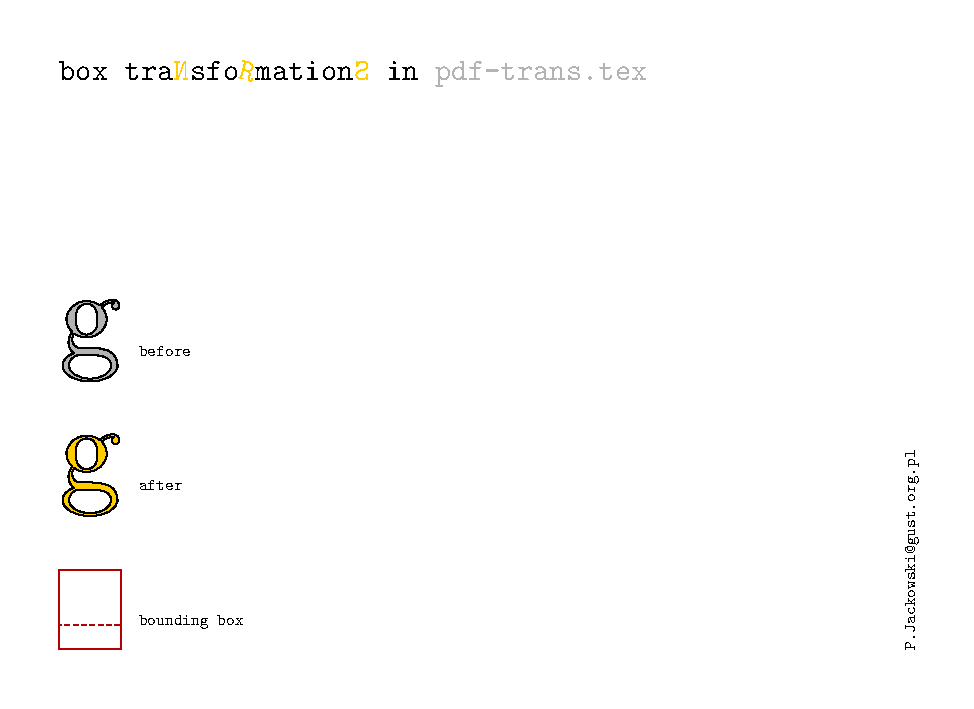
\includegraphics[bb= -25 -25 180 225,scale=.71,clip=true]{example.1}\hfill
  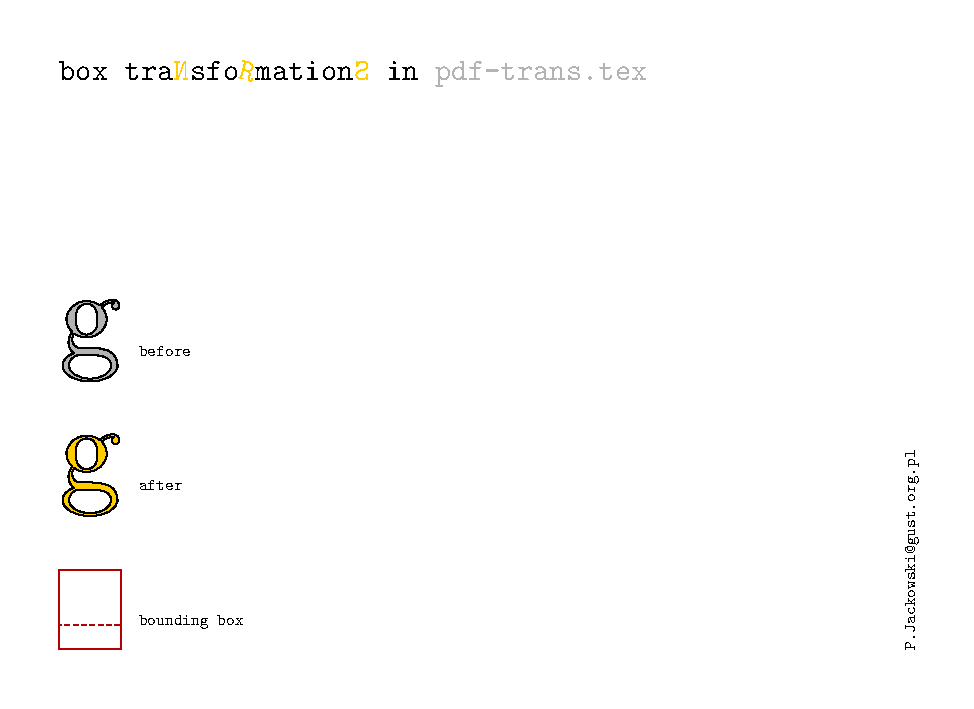
\includegraphics[bb = 10 -25 175 225,scale=.71,clip=false]{example.5}
  \caption{The original (left) and the with \exteps modified picture
    (middle). To the right there is one without the grid and the dot at the
    origin.}
  \label{fig:orig-and-mod}
\end{figure}

\clearpage
\subsection{Settings}
\label{sec:settings}

The parameters of the settings and their defaults can be seen the
table below\bigskip.

\noindent\begin{tabularx}{\linewidth}{llp{2cm}<\trr X}
  \toprule
  Parameter & Type & Default & Description\\
  \midrule
  angle & numeric & 0 & The counterclockwise rotation of the EPS figure.\\
  clipping\footnotemark & boolean & false & If true, the EPS figure is
  clipped to its bounding box.\\
  clippath & path & Bounding box of the EPS file & Path to which the
  EPS picture is clipped, if the \emph{clipping} switch is \emph{true.}\\
  base & pair & (0,0) & The offset of the lower left corner of the EPS
  picture.\\
  scale & pair & (1,1) & The scaling of the picture.\\
  width & numeric & No default & Specify the width of the picture;
  overrules the scale setting.\\
  height & numeric & No default & Specify the height of the picture;
  overrules the scale setting.\\
  grid & boolean & false & If true a grid is draw on top of the
  picture; mostly (only?) meant to help when drawing on top of the EPS
  figure.\\
  gridstep & numeric & 10 & The distance in percent between the lines
  of the grid.\\
  gridllx & numeric & 0 & The x-part of the lower left corner of the grid; in pct \\
  gridlly & numeric & 0 & The y-part\\
  gridurx & numeric & \emph{full width} & The x-part of the upper rightt corner of the grid\\
  gridury & numeric & \emph{full height} & The y-part\\
  \bottomrule
\end{tabularx}
\footnotetext{In version \oldstylenums{0.1} named \emph{clip}}

\subsection{Special values}
\label{sec:special-values}

\texttt{begineps} saves the original bounding box of the EPS picture
in the values \texttt{llx}, \texttt{lly}, \texttt{urx} and
\texttt{urx}. These values can be used in the settings, and for
drawing commands. Furthermore a numeric value \texttt{pct} is set.
This is a length that is one percent of the width of the picture.

If for instance one wants the picture to be placed at the same place on
the page as the original picture it is simply typing
\begin{lstlisting}
  base:=(llx,lly);
\end{lstlisting}
between \texttt{begineps} and \texttt{endeps}.

\subsection{Drawing commands}
\label{sec:drawing-commands}

When \texttt{begineps} is called a special picture,
\texttt{epspicture}, is created. To draw on this picture, and whence
drawing on the EPS picture the special commands \texttt{epsdraw},
\texttt{epsfill}, \texttt{epsfilldraw}, \texttt{epsdrawdot} and
\texttt{epslabel} are defined. They work as the normal drawing
commands, but now adds to the \texttt{epspicture}. 

At \texttt{endeps} the \texttt{epspicture} is scaled, rotated and
translated in the same way as the included EPS figure.

\subsection{Clipping the EPS picture}
\label{sec:clipping-eps-picture}

From version \oldstylenums{0.2} it is possible to do advanced clipping of the EPS
picture.

This is done by specifying the path \emph{clippath} along which the
EPS picture is to be clipped, and setting \emph{clipping} to
\emph{true}.

A minor example and the result in \fref{fig:clipped}:
\lstinputlisting[firstline=37,lastline=44]{example.mp}

\begin{figure}[tb]
  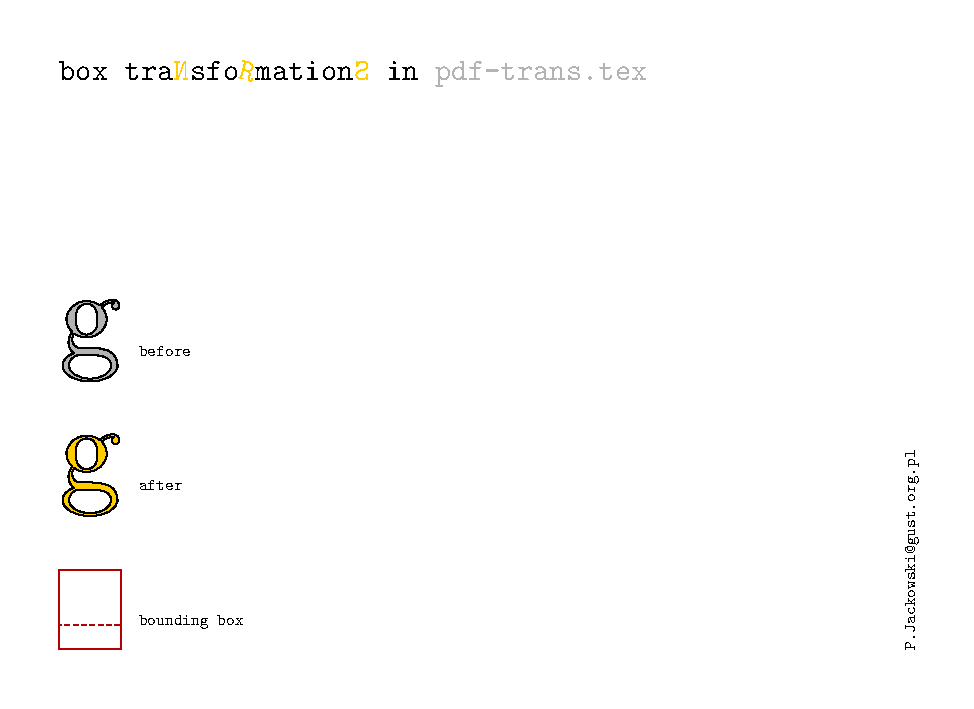
\includegraphics[scale=.71]{example.3}\hfill
  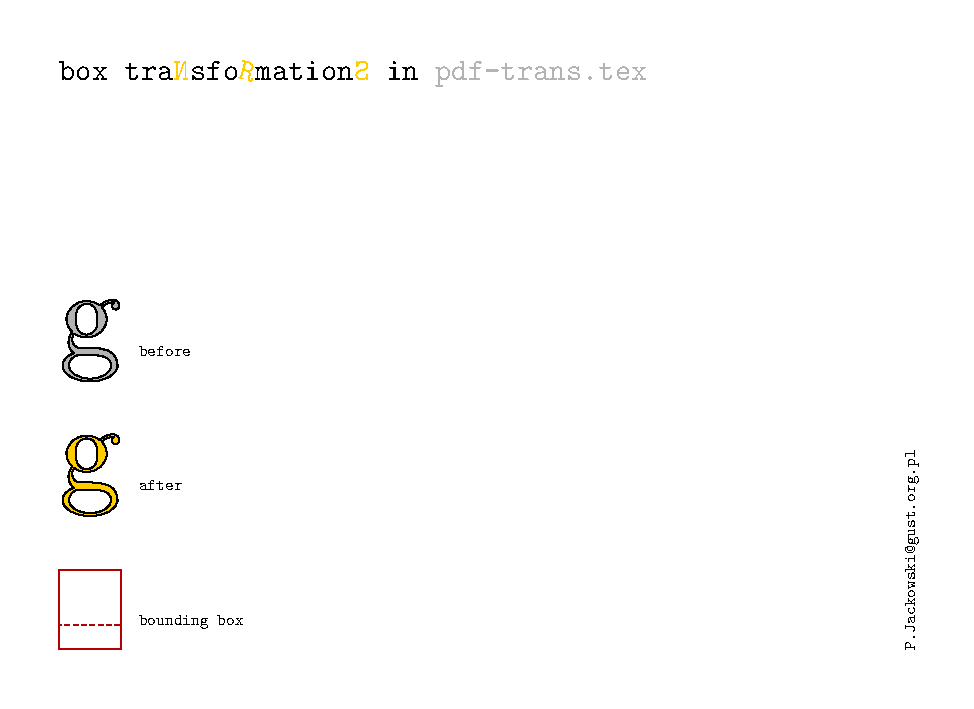
\includegraphics[bb = 30 -2 175 225,,scale=.71]{example.2}\hfill
  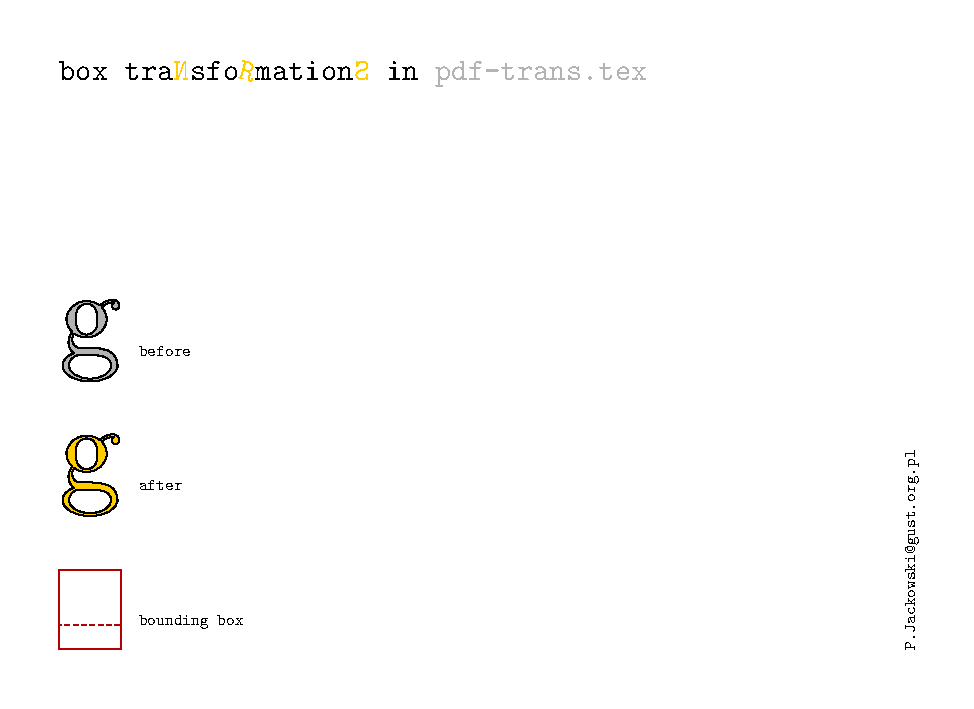
\includegraphics[bb = 30 -2 175 225,,scale=.71]{example.4}
  \caption{The clipped picture to the right, and the original with a
    grid to the left. The clippath is marked with blue. The picture in
    the midlle is created by keeping the blue line on top of the
    clipped picture.}
  \label{fig:clipped}
\end{figure}

Please note that this does not clip the \texttt{epspicture}.
You can do this manually by specifying
\begin{lstlisting}
  clip epspicture to clippath;
\end{lstlisting}
or
\begin{lstlisting}
  setbounds epspicture to clippath;
\end{lstlisting}

The section about the grid~\vpageref{sec:grid} also provides an
example of the clipping commands.

\newpage
\subsection{The grid}
\label{sec:grid}
It is possible to finetune the settings og the grid, for instance when
clipping the picture. The example below shows the impact of setting
the values of \texttt{gridstep}, \texttt{gridllx}, \texttt{gridlly},
\texttt{gridurx}, and \texttt{gridury}. The result can be seen in
\fref{fig:grid}.

\lstinputlisting[firstline=55,lastline=69]{example.mp}

\begin{figure}[tbp]
  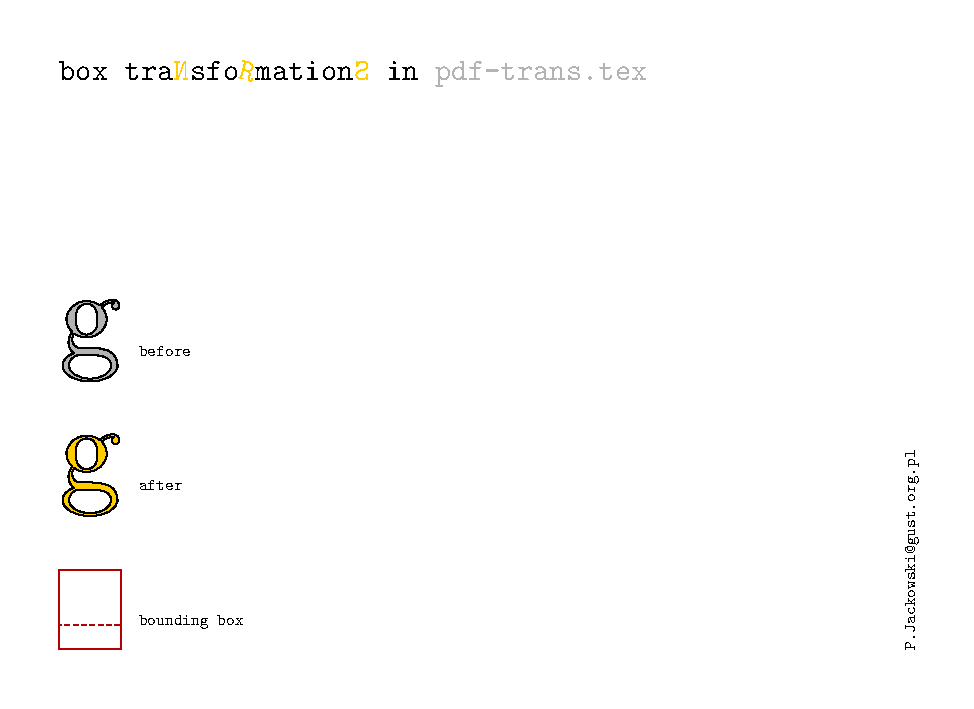
\includegraphics[scale=.71]{example.6}
  \caption{The picture with the finetuned grid, and some clipping.}
  \label{fig:grid}
\end{figure}

\section{Limitations of \exteps}
\label{sec:limitations}
\begin{itemize}
\item \exteps only looks at the first line in the document
  that says \\\verb|%%BoundingBox:|~\dots 
  
  Thus it will cause trouble if this line does not provide the
  bounding box; some PostScript drivers may write
  \verb|%%BoundingBox: (atend)|. This is not supported.
  
\item As all of the graphics inclusion is done with \MP, it is limited
  by \MP's memory capacity. More specific on the string pool size.
  
  Read more about this problem, and about the \emph{delfin} workaround
  perl script in \appendixname~\vref{sec:large-eps-files}

\item As the module makes it possible to include external EPS pictures
  it may not be possible to use the output with \textsc{pdf}\TeX.

  A way to get around this is to use the program epstopdf.

  epstopdf is  located on CTAN at\\
  \url{http://tug.ctan.org/tex-archive/support/epstopdf/}.
  
  Another possible work-around for this is to use the program
  purifyeps to ``clean up'' the PostScript picture.
  
  purifyeps is located on CTAN at\\
  \url{http://tug.ctan.org/tex-archive/support/purifyeps/}.
  
  Yet another work-around is to use the program pstoedit to generate
  \MP\ code form EPS files and include this into your \MP\ file.

  See \url{http://www.pstoedit.net/pstoedit/}.
\end{itemize}


\section{Changes}
\label{sec:changes}

\addtocontents{toc}{\setcounter{tocdepth}{1}}
\subsection{From version \mbox{\oldstylenums{0.1}} to \mbox{\oldstylenums{0.2}}}
\label{sec:from-version-0.1-to-0.2}

\begin{itemize}
\item Adding advanced clipping, see \fref{sec:clipping-eps-picture}.
\item Renaming the \emph{clip} switch to \emph{clipping}.
\item Eliminating the \verb|showpage| ``problem'' in version \oldstylenums{0.1}.
\end{itemize}

\subsection{From version \mbox{\oldstylenums{0.2}} to \mbox{\oldstylenums{0.3}}}
\label{sec:from-version-0.2-to-0.3}

\begin{itemize}
\item Improvement of the grid drawing commands. The grid is now drawn
  \emph{after} the scaling of the picture.
\item Introducing a workaround for large files. This includes a Perl
  script.
\end{itemize}

\section{Comments and Bug Reports}
\label{sec:comments-bug-reports}

All comments, questions and bug reports, both on the module itself as
well as this document may be sent to Palle J�rgensen,
\href{mailto:hamselv@pallej.dk}{hamselv@pallej.dk}.

\section{This document}
\label{sec:this-document}

\textcopyright\ \the\year\ by Palle J�rgensen.\\  The license of this
document is GNU General Public License. Source of this document and the
used example can be found at \url{http://pallej.dk/exteps/}.

\clearpage
\appendix
\section{Source code of \exteps}
\label{sec:source-code-exteps}

\lstinputlisting[firstline=22,extendedchars=true]{exteps.mp}

\clearpage
\section{Large EPS files}
\label{sec:large-eps-files}

In case of a too large EPS file, the \exteps module causes an error
message from \MP, due to the limited memory capacity of \MP.

The error message looks somewhat like this:

\begin{verbatim}
camel25:~/tmp% mpost et.mp
This is MetaPost, Version 0.641 (Web2C 7.5.2)
(/usr/local/TeX/texmf/web2c/cp8bit.tcx)
(et.mp (/users/pallej/texmf/metapost/exteps.mp)
Inserting sk.eps into et.1
! MetaPost capacity exceeded, sorry [pool size=476396].
<read>

<forever> __eps__currentline:=readfrom.file;
                                            exitunless.__eps__currentline<>E...

endeps->...<>EOF;special.__eps__currentline;endfor
                                                  .fi.special"%%EndDocument:...
l.14      endeps
\end{verbatim}
A workaround for this problem is to set the value \texttt{largefile}
to \texttt{true}:
\begin{lstlisting}
  largefile:=true;
\end{lstlisting}

\exteps now writes 
\begin{lstlisting}
  %% MetaPost exteps large file->file.eps
\end{lstlisting}
into the \MP\ output file. Afterwards one must run the Perl script
\delfin onto the \MP\ output file.

First run \MP:
\begin{verbatim}
This is MetaPost, Version 0.641 (Web2C 7.5.2)
(/usr/local/TeX/texmf/web2c/cp8bit.tcx)
(et.mp (/users/pallej/texmf/metapost/exteps.mp)
exteps notification:  File sk.eps not inserted into et.1
                      Run 'delfin et.1' to insert sk.eps
                      This is caused by setting 'largefile:=true'
[1] )
1 output file written: et.1
Transcript written on et.log.
camel25:~/tmp%
\end{verbatim}

and then \delfin
\begin{verbatim}
camel25:~/tmp% delfin et.1
This is delfin version 0.1
Delfin, the Exteps Large File INserter
Inserting sk.eps into et.1
camel25:~/tmp%
\end{verbatim}

It is possible to turn off the \exteps notification; just set the
(global) value \texttt{extepsverbose} to false
\begin{lstlisting}
  extepsverbose = false;
\end{lstlisting}

If you are unable to use the \delfin program, it is still possible
to do the finishing. Just open the \MP\ output file in your favourite
editor, and replace the line mentioned above with the entire EPS file.

\subsection{Using \delfin}
\label{sec:delfin-program}
Usage of the \delfin program:
\begin{verbatim}
delfin [options] file.n [file.m [file.l ... ]]
Options:
    -h  Print this message end exit
    -q  Be quiet
    -v  Display version and license and exit
    -V  Display version number and exit

\end{verbatim}

\subsection{Source of \delfin}
\label{sec:source-delfin}

\lstinputlisting[lastline=1,extendedchars=true,language=perl]{delfin}
[license stuff etc.]%\vskip-\baselineskip
\lstinputlisting[firstline=31,extendedchars=true,language=perl]{delfin}

\end{document}

%%% Local Variables: 
%%% mode: latex
%%% TeX-master: t
%%% End: 
